
\documentclass[xcolor=x11names,compress]{beamer}

\usepackage[utf8]{inputenc}
\usepackage[portuguese]{babel}
\usepackage{lmodern}
\usepackage[absolute,overlay]{textpos} 
\newenvironment{reference}[2]{% 
  \begin{textblock*}{\textwidth}(#1,#2) 
      \footnotesize\it\bgroup\color{red!50!black}}{\egroup\end{textblock*}} 
\title{Segurança básica de redes Wi-Fi}
\author[Lopez. V.L.O]{Víctor Orozco}
\date{\today}

%% Beamer Layout %%%%%%%%%%%%%%%%%%%%%%%%%%%%%%%%%%
\useoutertheme[subsection=false,shadow]{miniframes}
\useinnertheme{default}
%\usefonttheme{umbc2}
\usepackage{palatino}

%\setbeamerfont{title like}{shape=\scshape}
%\setbeamerfont{frametitle}{shape=\scshape}
%\setbeamerfont{structure}{family=\rmfamily,series=\bfseries} 

\setbeamercolor*{lower separation line head}{bg=DeepSkyBlue4} 
\setbeamercolor*{normal text}{fg=black,bg=white} 
\setbeamercolor*{alerted text}{fg=red} 
\setbeamercolor*{example text}{fg=black} 
\setbeamercolor*{structure}{fg=black} 
 
\setbeamercolor*{palette tertiary}{fg=black,bg=black!10} 
\setbeamercolor*{palette quaternary}{fg=black,bg=black!10} 

\renewcommand{\(}{\begin{columns}}
\renewcommand{\)}{\end{columns}}
\newcommand{\<}[1]{\begin{column}{#1}}
\renewcommand{\>}{\end{column}}
%%%%%%%%%%%%%%%%%%%%%%%%%%%%%%%%%%%%%%%%%%%%%%%%%%


\begin{document}
\begin{frame}
\begin{center}

\includegraphics[width=0.3\linewidth]{./Pictures/security}
\end{center}
\titlepage
\end{frame}

\begin{frame}
\frametitle{Agenda}
\tableofcontents
\end{frame} 

\section{Segurança}
\begin{frame}{Segurança}
\begin{figure}[tbph]
\centering

\includegraphics[width=0.3\linewidth]{./question}
\label{fig:question}
\end{figure}
\end{frame}

\begin{frame}{Segurança}
\begin{itemize}
\item Em um sentido amplio a segurança significa proteger os nossos ativos
\begin{itemize}
\item Proteger os nossos sistemas contra atacantes
\item Proteger o nosso prédio contra desastres naturais
\item Proteger a nossa carteira de roubos na boate
\end{itemize}
\end{itemize}
\end{frame}

\begin{frame}{Segurança informação}
\begin{itemize}
\item Dependendo do contexto assim tem que ser as medidas de segurança
\begin{itemize}
\item Ativos físicos: Computadores, carros
\item \textbf{Ativos lógicos: Arquivos de dados, código fonte de aplicativos}
\item Ativos humanos: Seres humanos a base de qualquer negocio
\end{itemize}
\end{itemize}
\end{frame}

\section{Redes sem fio}
\begin{frame}{Redes sem fio}
Sistemas de transmissão
\begin{itemize}
\item \textbf{Rádio}
\item Infravermelho
\item Laser
\end{itemize}
\end{frame}

\begin{frame}{Tipos de ondas}
\begin{itemize}
\item \textbf{Direcional}
\item Não direcional
\end{itemize}
\end{frame}

\begin{frame}{Tecnologias}
\begin{itemize}
\item Bluetooth
\item ZigBee
\item WiMax
\item \textbf{Hotspot}
\item \textbf{Wi-Fi}
\end{itemize}
\begin{center}
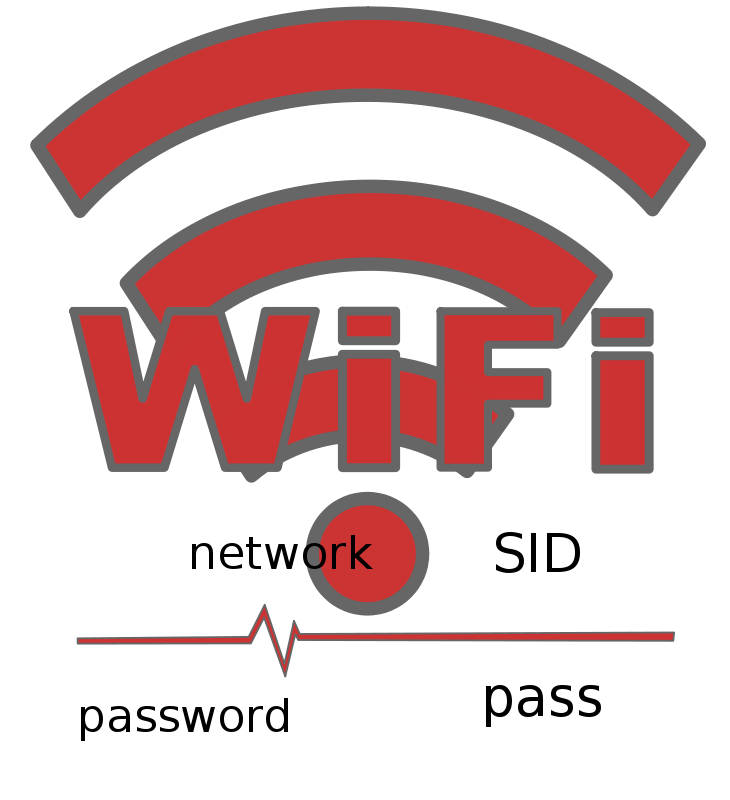
\includegraphics[width=0.3\linewidth]{./Pictures/free_wifi}
\end{center}
\end{frame}


\begin{frame}{Modelos de rede}
\begin{itemize}
\item Fechados
\begin{itemize}
\item Wpan (Bluetooth)
\item \textbf{Wlan (Wi-Fi)}
\end{itemize}
\item Abertos
\begin{itemize}
\item Wman (Rede de redes)
\item Wwan (GSM, LTE, 3G, etc.)
\end{itemize}
\end{itemize}
\end{frame}

\section[Wi-Fi]{Wi-Fi}
\begin{frame}{Problemas}
\pause
\begin{itemize}[<+->]
\item A área de cobertura Wi-Fi excede os limites físicos da nossa sala
\item As pessoas "ruins" tentam aproveitar estes "excedentes" pra invadir a rede
\item Melhor cenário = pegar internet de graça
\item Pior cenário = pegar informação privada
\end{itemize}
\end{frame}

\begin{frame}{Terminologia}
\begin{itemize}
\item {Claridade da sinal:} Potencia, distancia, interferências, linha de visão;
\item {ESSID:} Nome da rede;
\item {BSSID:} Endereço MAC da rede;
\item {Beacon:} Anuncio da presença de uma rede Wi-Fi;
\item {Canais:} Divisões da sinal (2.4/5 Ghz) em un numero de bandas;

\item {Cifrado+Autenticação:} OPN, WEP, WPA/WPA2 (CCMP, WRAP, TKIP, WEP, WEP40, WEP104, MGT, SKA, PSK) 
\end{itemize}
\end{frame}

\begin{frame}{WEP}
\begin{itemize}
\item Não foi criado por expertos em cifrado e segurança.
\item Algoritmo RC4 é a principal debilidade.
\item 24 bits – precisam-se menos de 5000 pacotes pra ter um 50\% de probabilidade de pegar a senha.
\item Alem disso não existe uma comprobação de integridade de pacotes apropriada. (CRC32 linearidade não criptográfica).
\end{itemize}
\end{frame}

\begin{frame}{WPA/WPA2}
\begin{itemize}
\item Solução temporal da Wi-Fi Alliance.
\item 802.11i da IEEE  = WPA2
\item Autenticação mediante PSK pra entornos domésticos (senha) e suporte pra servidores de autenticação (RADIUS).
\item A principal diferença é o algoritmo WPA-TKIP(baseado RCA4) e WPA2-CCMP(baseado em AES).
\item A vulnerabilidade do protocolo não radica no algoritmo mas na senha (handshake), ja que se o handshake é capturado e a senha fraca ...
\end{itemize}
\end{frame}

\begin{frame}{Tipos de ataque}
Passivos
\begin{itemize}
\item Packet sniffing (captura de pacotes)
\item Analise de padrões de trafego
\end{itemize}
\pause
Ativos
\begin{itemize}
\item Suplantação (clonar uma PC)
\item Rogue AP/Evil twin (clonar o AP para receber a autenticação)
\item Modificação de pacotes (MTIM)
\item Reautuação - injeção de pacotes pra simular trafego legitimo
\item Denial of service - só pra incomodar
\item Ataques de dicionario / força bruta
\end{itemize}
\end{frame}



\section{Demo}
\begin{frame}{Demo}
\begin{itemize}
\item Ferramentas: Funtoo Linux, Aircrack
\item airodump: Sniffing de pacotes.
\item aireplay: Injeção de pacotes (aumentar o trafego e a velocidade do ataque).
\item aircrack: A partir dos pacotes recolhidos ele faz uma analise estatística (WEP), força bruta/dic (WPA)
\end{itemize}
\end{frame}

\begin{frame}{Demo WEP}
\begin{enumerate}
\item Ativar o modo monitor na placa.
\item Descobrir os detalhes das redes por perto.
\item Iniciar a captura da rede desejada (BSSID, ESSID, canal)
\item Injetar trafego baseado nos dados capturados.
\item Pegar a senha WEP
\pause
\item Barbada!
\end{enumerate}
\end{frame}


\begin{frame}{Demo WEP}
\begin{center}
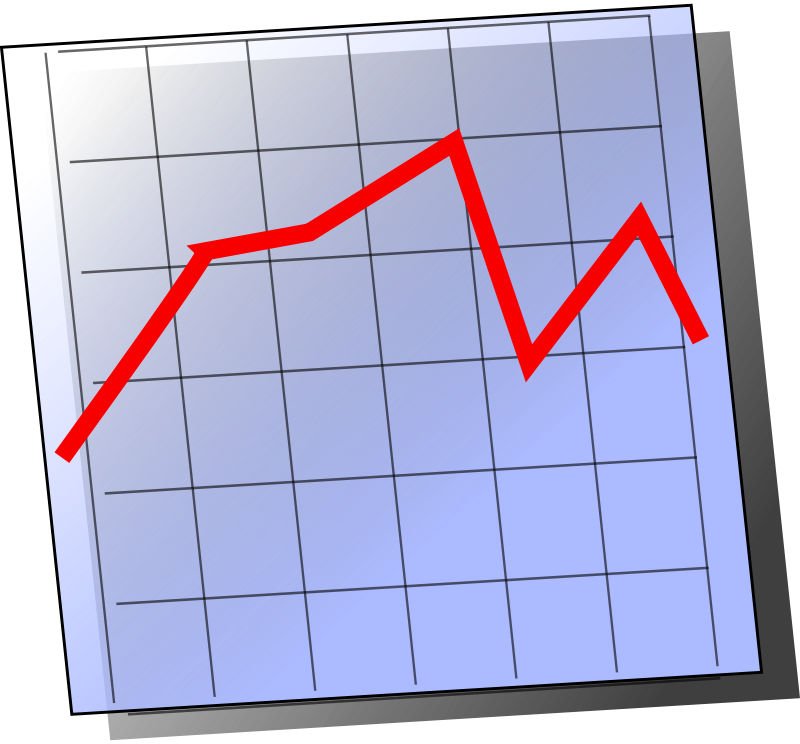
\includegraphics[width=0.5\linewidth]{./Pictures/wep}
\end{center}
\end{frame}

\begin{frame}{Demo WPA}
\begin{enumerate}
\item Ativar o modo monitor na placa.
\item Descobrir os detalhes das redes por perto.
\item Iniciar a captura da rede desejada (BSSID, ESSID, canal)
\item Forçar ou aguardar por um handshake.
\item Atacar o handshake capturado com dicionario.
\pause
\item Não tão barbada . . .
\end{enumerate}
\end{frame}


\begin{frame}{Demo WPA}
\begin{center}
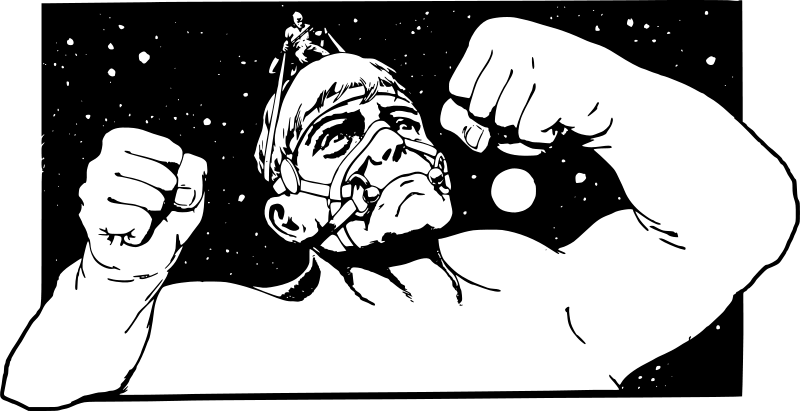
\includegraphics[width=0.5\linewidth]{./Pictures/wpa}
\end{center}
\end{frame}


\section[Segurança]{¿Como segurar uma rede sem fio?}
\begin{frame}{WPA/WPA2}
Segurança nível 0
\begin{itemize}
\item Mudar a senha original do AP.
\item Mudar o SSID original.
\item WPA-PSK+senha segura, nunca WSP.
\end{itemize}
\pause
Segurança nível 1
\begin{itemize}
\item Ocultar SSID (deshabilitar broadcast SSID) - Engenharia social
\item Configurar filtrado MAC - Mac spoofing
\item Mudar as senhas de forma regular - Furto de dispositivos, dicionario
\item Desabilitar DHCP - Uma vez dentro da rede é a ultima barrera de comunicação
\item Scheduler WLAN/ Desligar - Dicionario
\item Diminuir a sinal do roteador ;-)
\end{itemize}
\end{frame}

\begin{frame}{Obrigado!}
\begin{itemize}
\item tuxtor@shekalug.org
\item http://tuxtor.shekalug.org
\item http://github.com/tuxtor/slides
\end{itemize}
\begin{center}
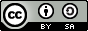
\includegraphics[width=0.1\linewidth]{Pictures/cclogo}
\\
This work is licensed under a Creative Commons Attribution-ShareAlike 3.0 Brazil License.
\end{center}
\end{frame}


\section{Referencias}
\begin{frame}[allowframebreaks]{Referencias}
    \bibliographystyle{sbc}
    \bibliography{small}
\end{frame}
\end{document}